\chapter{Kullback-Leibler Divergence}

\section{Space Worms}
We’re a group of scientists visiting the vast outer-space and we discovered some space worms. These space worms have varying number of teeth. Now we need to send this information back to earth, but sending information from space to earth is expensive. So we need to represent this information with a minimum amount of information. A great way to do this is, instead of recording individual numbers, we draw a plot where $X$ axis is different numbers of teeth that has been observed and make $Y$ axis the probability of seeing a worm with x many teeth (that is, number of worms with $x$ teeth / total number of worms). We have converted our observations to a distribution.

This distribution is efficient than sending information about individual worms, but we can do better. We can represent this distribution with a known distribution, so that we only need to send even fewer pieces of information to recover true data. But how do we know which distribution explains the true distribution better? Well that’s where the Kullback-Leibler (KL) divergence comes in.

\emph{Essentially KL divergence is a way of measuring the matching between two distributions}. So we could use the KL divergence to make sure that we matched the true distribution with some simple-to-explain and well-known distribution well.

Say we have 100 worms. And we have following types of worms in following amounts:

\begin{table}[htbp]
\centering
\begin{tabular}{|c|c|c|}
\hline
Teeth & Frequency & Probability\\
\hline
\hline
0 & 2 & 0.02 \\
1 & 3 & 0.03 \\
2 & 5 & 0.05 \\
3 & 14 & 0.14 \\
4 & 16 & 0.16 \\
5 & 15 & 0.15 \\
6 & 12 & 0.12 \\
7 & 8  & 0.08 \\
8 & 10 & 0.1  \\
9 & 8  & 0.08 \\
10 & 7 & 0.07 \\
\hline
\end{tabular}
\end{table}

Figure~\ref{fig:worms} shows what it looks visually.

\begin{figure}[htpb]
  \centering
  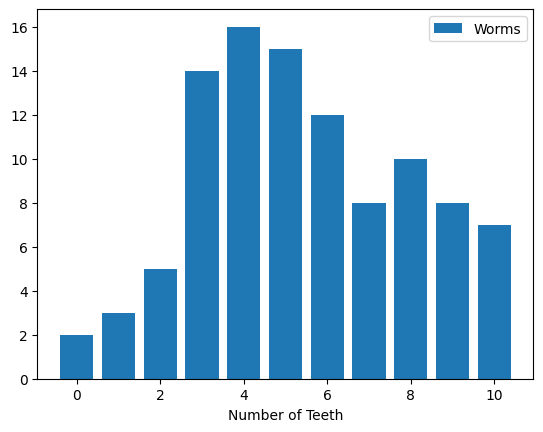
\includegraphics[width=0.5\linewidth]{figures/worms_distro}
  \caption{Recorded distribution of worms teeth.}
  \label{fig:worms}
\end{figure}

\subsection{Model with a Uniform Distribution}
A uniform distribution has only a single parameter; the uniform probability; the probability of a given event happening.
\begin{equation*}
p_{uniform}=1/total events=1/11 = 0.0909
\end{equation*}

\begin{figure}[htpb]
  \centering
  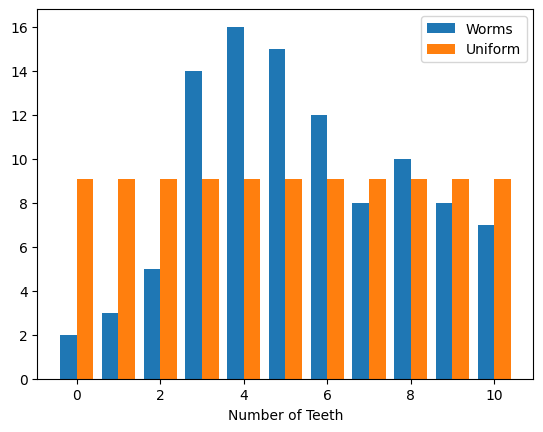
\includegraphics[width=0.5\linewidth]{figures/worms_uniform}
  \caption{What the uniform distribution and the true distribution side-by-side looks like.}
  \label{fig:worms_uniform}
\end{figure}

\subsection{Model with a Binomial Distribution}
Let us first calculate the expected number of teeth for the worms. It would be,

\begin{equation*}
  n = \sum_i i*p_i = 5.44
\end{equation*}

With mean known, we can calculate $p$ where, $mean=np\implies p=\frac{5.44}{10}=0.544$. Note than $n$ is the maximum number of teeth observed from the population of worms. %You might ask why we did not choose n to be the total number of worms (that is 100) or total number of events (that is 11). We will soon see the reason. With that, we can define probabilities of any number of teeth as follows.

\begin{figure}[htpb]
  \centering
  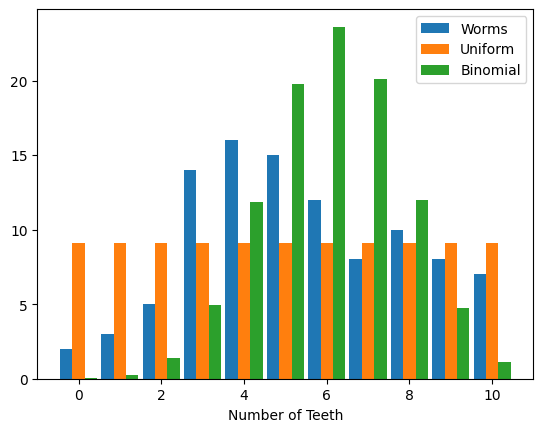
\includegraphics[width=0.5\linewidth]{figures/worms_uniform_binomial}
  \caption{This is what a comparison between the true distribution and the binomial distribution looks like.}
  \label{fig:worms_binomial}
\end{figure}

\subsection{How do we quantitatively decide which ones the best?}

This is where the KL divergence comes in. KL divergence is formally defined as follows.
\begin{equation}
  D_{KL} = \sum_{i=1}^{N} p(x_i)\log\left(\cfrac{p(x_i)}{q(x_i)}\right)
\end{equation}

Here $q(x)$ is the approximation and $p(x)$ is the true distribution we’re interested in matching $q(x)$ to. Intuitively this measures the how much a given arbitrary distribution is away from the true distribution. If two distributions perfectly match, $D_{KL}e = 0$ otherwise it can take values between 0 and $\infty$. Lower the KL divergence value, the better we have matched the true distribution with our approximation.

Inded if $q(x_i)$ is higher than $p(x_i)$ the log term produces a negative value. On the other hand if $q(x_i)$ is always smaller than $p(x_i)$ this component will produce positive values. This will be zero only if $p(x_i)=q(x_i)$. Then to make this an expected value, you weight the log component with $p(x_i)$. This means that, matching areas where $p(x_i)$ has higher probability is more important than matching areas with low $p(x_i)$ probability.

\subsection{Computing KL Divergence}
Let us now compute the KL divergence for each of the approximate distributions we came up with. First let’s take the uniform distribution.
\begin{equation*}
D_{KL}(True||Uniform) = 0.136
\end{equation*}

Now for the binomial distribution we get,
\begin{equation*}
D_{KL}(True||Binomial) = 0.427
\end{equation*}

Though the uniform distribution appears to be simple and very uninformative where the binomial distribution carries more subtlety, the uniform distribution matches the true distribution better than the binomial distribution. Therefore, this teaches us the importantness of why we should not trust our instincts alone !

%\section{Reparameterization Trick}
%Here we will understand the reparameterization trick used by Kingma and Welling (2014) to train their variational autoencoder.
%
%Assume we have a normal distribution q
% that is parameterized by θ
%, specifically qθ(x)=N(θ,1)
%. We want to solve the below problem
%minθEq[x2]
%This is of course a rather silly problem and the optimal θ
% is obvious. We want to understand how the reparameterization trick helps in calculating the gradient of this objective Eq[x2]
%.
%
%One way to calculate ∇θEq[x2]
% is as follows
%∇θEq[x2]=∇θ∫qθ(x)x2dx=∫x2∇θqθ(x)qθ(x)qθ(x)dx=∫qθ(x)∇θlogqθ(x)x2dx=Eq[x2∇θlogqθ(x)]
%For our example where qθ(x)=N(θ,1)
%, this method gives
%∇θEq[x2]=Eq[x2(x−θ)]
%Reparameterization trick is a way to rewrite the expectation so that the distribution with respect to which we take the expectation is independent of parameter θ
%. To achieve this, we need to make the stochastic element in q
% independent of θ
%. Hence, we write x
% as
%x=θ+ϵ,ϵ∼N(0,1)
%Then, we can write
%Eq[x2]=Ep[(θ+ϵ)2]
%where p
% is the distribution of ϵ
%, i.e., N(0,1)
%. Now we can write the derivative of Eq[x2]
% as follows
%∇θEq[x2]=∇θEp[(θ+ϵ)2]=Ep[2(θ+ϵ)]
%Now let us compare the variances of the two methods; we are hoping to see that the first method has high variance while reparameterization trick decreases the variance substantially.
%
